\section{Methodology}
\label{sec:meth}


\subsection{Description of the data}
De dataset die gebruikt gaat worden om deze vragen te beantwoorden is een verzameling van troonredes sinds 1814. De gehele dataset bestaat uit 165 verschillende troonredes welke in totaal uit 219236 woorden bestaan, deze set zullen we vanaf nu het corpus noemen. Deze troonredes zijn terug te vinden op www.troonredes.nl~\citep{troonredes} . Om een duidelijker beeld te geven van de troonredes een korte uitleg van wat de troonredes nu precies zijn en waar ze vandaan komen. 

De troonrede wordt jaarlijks door de koning(in) uitgesproken op Prinsjesdag, de 3de dinsdag van september. voor 1904 werden de troonredes uitgesproken in de vergaderzaal van de 2de kamer. Sinds 1904 worden de troonredes voor de ridderzaal op het binnenhof in Den Haag uitgesproken. De troonrede wordt live uitgezonden op televisie en is na te lezen op de website van de Nederlandse overheid. De eerste troonrede werd in 1818 als een algehele toespraak voor de Staten-generaal gehouden. De troonredes worden vooral gebruikt om wets- en beleidsveranderingen door te geven, als beschouwing op het afgelopen jaar en de staat van het land. In recentere jaren heeft deze beschouwing zich ook uitgebreid naar gebeurtenissen door de hele wereld die invloed uitoefenen op de Nederlandse staat. Ook wordt sinds 1918 het regeerprogramma voor het komende jaar in de troonredes behandelt. Sinds 1848 worden de troonredes geschreven door ministers vanwege een grondwetsherziening waardoor de ministers verantwoordelijk werden voor al het doen en laten van de koning(in). Hiermee werd het kabinet verantwoordelijk voor de uitspraken die gedaan worden in de troonredes.~\citep{overheid} Dit zorgt ervoor dat de troonredes een beeld geven van wat de Nederlandse regering op dat moment belangrijk vindt.

\subsubsection{Missing data}
Er zijn verscheidene jaren waarvan er geen data beschikbaar is, dit doordat er niet elk jaar een troonrede gegeven is. Dit heeft verschillende redenen, zoals oorlogen, angst voor rellen, onvrede over het kabinet of gezondheidsredenen omtrent de koning(in). Dit zorgt ervoor dat niet elk jaar sinds 1818 wordt gerepresenteerd door een troonrede. Omdat de inhoud van de troonredes als verzamelde dataset wordt gebruikt heeft dit minimaal invloed op de uiteindelijke uitkomsten van het onderzoek dat er jaren missen. Door de missende jaren is het weergeven van de verschuiving in onderwerpen mogelijk niet volledig representatief, omdat er geen uitspraken gedaan kunnen worden over de missende jaren.
In tabel \ref{missing} een overzicht van de jaren waar geen troonredes van zijn en de reden dat er in die jaren geen troonrede is gegeven:
\newline
\newline
\begin{table}[htb]
\centering
\begin{tabular}{ll}
\toprule
{} &                       reden \\
Jaren     &                             \\
\midrule
1888-1890 &  Verhindering wegens ziekte en interne beleidsproblemen\\
\\
1905-1924 &         Eerste wereldoorlog en politieke instabiliteit\\
\\
1940-1947 &         Tweede wereldoorlog en politieke instabiliteit\\
\bottomrule
\end{tabular}
\caption{Missende troonredes}
\label{missing}
\end{table}

\subsubsection{Quality of the data}
Hier moet nog een deel komen over het feit of het ingescand is of ingetypt.

\subsection{Wat plotjes en tabelletjes}

De grafiek in figuur \ref{inhoud} geeft een beeld van de grootte van de troonredes over de jaren aan de hand van het aantal zinnen en paragrafen per jaar.

\begin{figure}[H]
\begin{center}
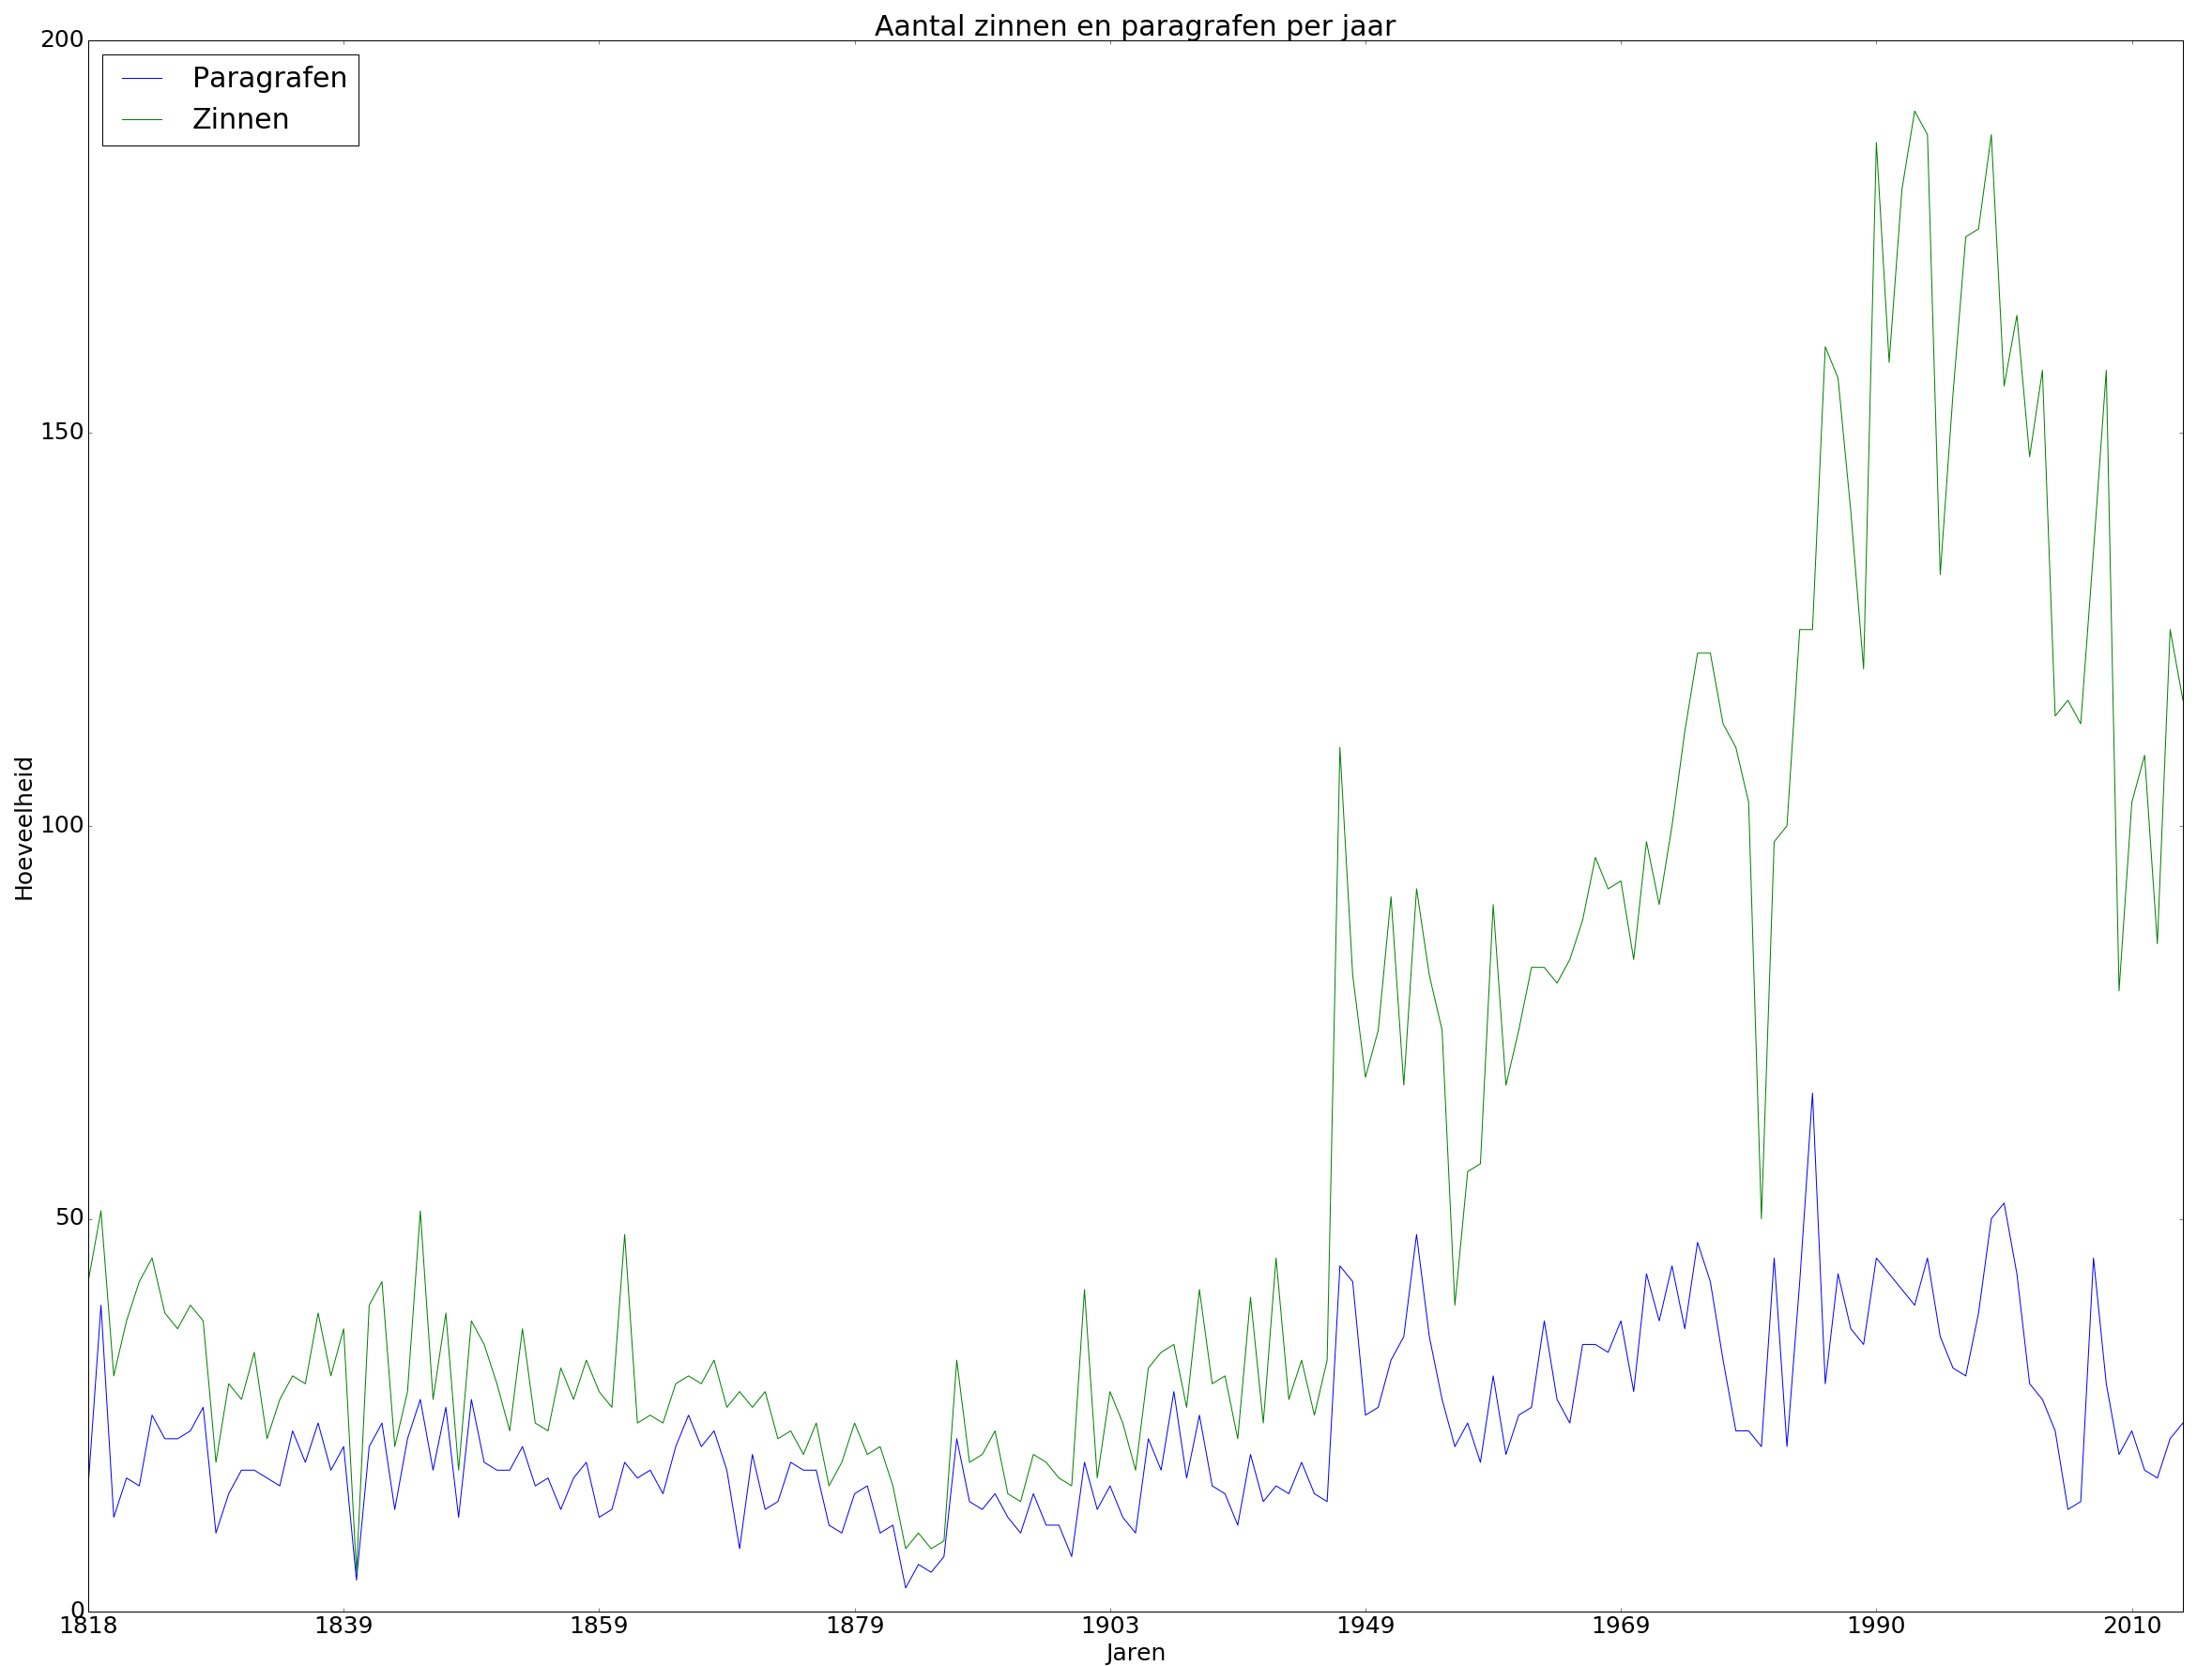
\includegraphics[width=1.2\textwidth]{fig/Inhoudverdeling}
\caption{\label{inhoud} Weergave van het aantal zinnen en paragrafen per jaar.}
\end{center}
\end{figure}



\pagebreak
\subsection{Methods}
Om uit het corpus te kunnen achterhalen of er overkoepelende onderwerpen zijn en wat deze mogelijk zijn wordt er gebruik gemaakt van tekstanalyse technieken. Specifiek wordt er gebruik gemaakt van POS-methodes en co-occurence aanpakken.~\cite{callon1991co}  

Allereerst wordt er met behulp van POS-methodes(Pattern of Speech) gekeken naar het volledige corpus. Deze methodes kijken naar het corpus als geheel en proberen hier patronen uit te halen. Er is specifiek gebruik gemaakt van "Pattern", een Python module, die getraind is voor Nederlandse tekst. Deze module is getraind op verschillende soorten Nederlandse teksten en kan woorden uit de tekst onderverdelen in verschillende categorieën, zoals lidwoorden en zelfstandige naamwoorden. Met behulp van deze module is het corpus gefilterd zodat enkel de zelfstandige naamwoorden zijn overgebleven. De reden dat we enkel zelfstandige naamwoorden gebruiken is het feit dat deze representatief zijn voor de tekst, omdat vanuit de zelfstandige naamwoorden afgeleid kan worden wat het doel en inhoud van de tekst is.

Hierna wordt de data van de troonredes gelemmatiseerd. Hierdoor worden de woorden herleid tot hun lemma(stam), waardoor ze kunnen worden geanalyseerd als één term. Enkele voorbeelden hiervan: "steden" wordt herleid tot "stad" en "mensen" tot "mens". Doordat alle woorden hierdoor tot de stam zijn herleidt is er een duidelijk beeld van alle unieke woorden die gebruikt worden. Hierdoor zal de relatie tussen woorden sneller duidelijk worden, omdat er nu geen onderscheid wordt gemaakt tussen de verschillende vervoegingen van unieke woorden. Met behulp van deze gelemmatiseerde termen wordt een co-occurence matrix opgesteld. Deze matrix wordt aangemaakt door bij te houden hoe vaak een combinatie van 2 termen samen in een paragraaf voorkomen. De matrix geeft uiteindelijk voor alle combinaties van 2 termen de frequentie dat ze samen in een paragraaf voorkomen weer.

Voor alle combinaties uit deze matrix wordt een nabijheidsscore berekend via de volgende definitie: 

 $$S(W_1,W_2)\equiv^{\mathrm{def}\frac{\sum_{c\epsilon W\setminus{W_1,W_2\},PMI(W_1,c)>0}}min(PMI(W_1,c),PMI(W_2,c))}{\sum_{c\epsilon W\{W_1,W_2\},PMI(W_1,c)>0}PMI(W_1,c)}}$$ 

Hierbij is het doel om uit te vinden welke termen relevant zijn en hoe deze zich over tijd met andere termen associëren. De score geeft het verwantschap tussen twee termen "W1" \& "W2" aan. Dit verwantschap wordt bepaald aan de hand van PMI(Pointwise Mutual Information) tussen twee termen \citep{bouma2009normalized}. Hierbij geeft de PMI tussen twee termen "X" \& "Y" aan hoeveel de termen ons over elkaar kunnen vertellen. Hierbij gaat het om het verschil in de kans dat term "X" of "Y" individueel voorkomt in een paragraaf in de tekst en de kans dat termen "X" \& "Y" samen voorkomen in een paragraaf in de tekst. Wiskundig gezien wordt PMI als volgt berekend: 

$$PMI(X,Y)\equiv^{\mathrm{log}\frac{p(X,Y)}{p(X)}}$$

Hierbij is P(X,Y) de kans dat termen "X" \& "Y" samen in een paragraaf voorkomen en P(X) de kans dat term "X" in een paragraaf voorkomt. Dit wordt berekend door het aantal keer dat de term voorkomt in de tekst te delen door het aantal paragrafen. De PMI is een score die positief of negatief kan zijn. Goede collocatie paren van termen hebben een hoge PMI score omdat ze net iets minder samen voorkomen dan dat ze individueel voorkomen.  Een score van 0 betekent dat de termen onafhankelijk van elkaar zijn en er geen uitspraak gedaan kan worden over het voorkomen van term "X" als "Y" voorkomt en vice versa.

Deze vergelijking voor de nabijheidsscore maakt gebruikt van de termen uit het gehele corpus om context te bepalen. Hiervoor wordt voor elke combinatie termen (W1,W2) gekeken naar de woorden waarmee ze samen in een paragraaf voorkomen. De som van PMI(W,C) voor alle termen (C) uit het corpus waarvoor geldt dat PMI(W,C) \textgreater 0 wordt voor beide termen berekend. Dit betekent dus dat er enkel wordt gekeken naar combinaties van termen die onafhankelijk van elkaar zijn, met een score van 0, of  positief. Als hieruit volgt dat PMI(W1,C) gelijk is aan PMI(W2,C) kan men stellen dat als W1 in een paragraaf voorkomt W2 ook voorkomt en vice versa. Een nabijheidsscore van 0 geeft aan dat de woorden nooit samen in een paragraaf voorkomen. Aan de hand van deze score wordt een gewogen semantisch netwerk gevormd met de termen als nodes en de gewichten op de edges. Om de termen binnen dit netwerk te kunnen analyseren wordt gebruik gemaakt van een community detectie algoritme. Het specifieke algoritme dat gebruikt wordt is dat van~\cite{blondel2008fast}. Het doel van dit algoritme is om vanuit het gewogen netwerk clusters te vormen van samenhangende subsets van termen. Om ervoor te zorgen dat enkel de meest relevante termen worden meegegeven aan het community detectie algoritme is een drempelwaarde bepaald. Deze drempelwaarde geeft aan vanaf welke waarde voor de nabijheidsscore de co-occurence combinaties door het algoritme verwerkt worden. De drempelwaarde ligt tussen de 0 en 1 en wordt bepaald door vanaf 0 de score op te hogen. Dit is een handmatig proces waarbij de drempelwaarde is bereikt als er binnen het netwerk een component van meer dan twee nodes verdwijnt. Hiermee worden de zwak verbonden nodes uit het netwerk verwijderd. De drempelwaarde die gevonden is voor ons netwerk is θ=0.65. Het resulterende netwerk is door het community detectie algoritme verwerkt om de verschillende subsets te kunnen identificeren. Vanuit deze subsets zijn onderwerpen bepaald aan de hand van de termen die er onder vallen. Afhankelijk van de termen binnen deze clusters kunnen deze clusters gezien worden als indicatief voor onderwerpen/thema's binnen het corpus. Dit induceren van onderwerpen moet een overzicht geven van de verschillende termen die tot een onderwerp behoren en hoe sterk de samenhang is tussen termen binnen een onderwerp. Ook zou het een beeld moeten geven van de samenhang tussen verschillende onderwerpen. 
